Auf Basis der Dimensionierung der einzelnen Komponenten kann die Masse der Tragfläche abgeschätzt werden. Im Folgenden werden die Volumina bestimmt, um mithilfe der Dichte des jeweiligen Werkstoffes auf die Masse zu schließen. Mithilfe des CAD-Programms können die Volumina zeitsparend und exakt bestimmt werden. Dies ist besonders für komplizierte Geometrien, zum Beispiel für den Schaumkern der Haut hilfreich.
\subsubsection{Masse der Gurte}
Für den oberen und unteren Gurt ergeben sich folgende Werte: 
\begin{equation}
	V_{Gurt,o}=A_{Gurt,o}\cdot \left(l_{0}+l_{1}+l_{2}+l_{3}\right)\\
	=4,983\cdot 10^{-5}m^{3}
\end{equation}
\begin{equation}
	V_{Gurt,u}=A_{Gurt,u}\cdot \left(l_{0}+l_{1}+l_{2}+l_{3}\right)\\
	=4,98\cdot 10^{-5}m^{3}.
\end{equation}
 Im nächsten Schritt wird die Dichte der Faserverbundbauteile bestimmt. Sie errechnet sich gemäß der Mischungsregel nach \cite{item3} zu
\begin{equation}
	\rho_{Verbund}=\varphi\cdot\rho_{f}+\left(1-\varphi\right)\cdot\rho_{m}
	=1728\frac{kg}{m^{3}}.
\end{equation}
Gemäß dieser Formel sind die Dichten der Verbundbauteile unabhängig von den verwendeten Geweben und ihren Flächengewichten, solange das gleiche Fasermaterial und der gleiche Faservolumengehalt vorliegen. Damit ergeben sich die Massen der Gurte zu
\begin{equation}
	m_{Gurt,o}=V_{Gurt,o}\cdot\rho_{Verbund}=0,0861kg
\end{equation}
\begin{equation}
		m_{Gurt,u}=V_{Gurt,u}\cdot\rho_{Verbund}=0,086kg .
\end{equation}

\subsubsection{Masse des Stegs}
Unterteilt in den Anteil des Schaums und den des Verbundmaterials, ergeben sich für den Steg folgende Volumina:
\begin{equation}
	V_{Steg,Verb}=A_{Steg,Verb}\cdot\tilde{h_{i}}=1,813\cdot10^{-5}m^{3}
\end{equation}
\begin{equation}
	V_{Steg,Schaum}=A_{Schaum}\cdot\tilde{h_{i}}=4,953\cdot10^{-5}m^{3}.
\end{equation}
Für die jeweiligen Volumina folgt mit der Dichte $ \rho_{Verbund} $ und der Dichte des Schaums $ \rho_{Schaum}=35\frac{kg}{m^{3}} $:
\begin{equation}
	m_{Steg,Verb}=V_{Steg,Verb}\cdot\rho_{Verbund}=0,031kg
\end{equation}
\begin{equation}
		m_{Steg,Schaum}=V_{Steg,Schaum}\cdot\rho_{Schaum}=0,002kg
\end{equation}
Als Werkstoff für den Schaum steht Styrodur zur Verfügung. Laut Trendbericht aus dem Magazin \textit{Kunststoffe} in der Ausgabe 10/2008 \cite{item7}, beträgt die Dichte von extrudiertem Polystyrol-Hartschaumstoff (XPS) $ 25\frac{kg}{m^{3}} $ bis $ 45\frac{kg}{m^{3}} $. Für die Massenabschätzung wurde der Mittelwert angenommen.

\subsubsection{Masse der Haut}
Das Volumen des Schaumkerns der Haut beträgt 
\begin{equation}
	V_{Haut,Schaum}=A_{Haut,Schaum}\cdot l_{3}=6,143\cdot10^{-4}m^{3}.
\end{equation}
Mit der Dichte $ \rho_{Schaum} $ beträgt die Masse des Kerns
\begin{equation}
	m_{Haut,Schaum}=V_{Haut,Schaum}\cdot\rho_{Schaum}=0,022kg.
\end{equation}
Zur Bestimmung der Masse des Faserverbundanteils in der Haut wird die Länge der abgewickelten Hautschichten mit dem CAD-Programm bestimmt. Für die innere und die äußere Schicht ergeben sich:
\begin{equation}
	l_{Haut,innen}=346,46mm
\end{equation}
\begin{equation}
	l_{Haut,aussen}=367,83mm
\end{equation}
Die Dicke einer Schicht des Interglas 90070 Gewebes mit einer flächenbezogenen Masse von $ 80\frac{g}{m^{2}} $
berechnet sich nach \cite{item3} mit der Formel:
\begin{equation}
	t=n\cdot\frac{m}{Lb}\cdot\frac{1}{\varphi\cdot\rho_{f}}.
\end{equation}
Für eine Schicht, $ \varphi=0,4 $ und $ \rho_{f}=2550\frac{kg}{m^{3}} $ ist $ t_{Haut}=0,078mm $.
Die Breite entspricht Länge $ l_{3} $, damit ergibt sich das Volumen der inneren und äußeren Hautschicht zu:
\begin{equation}
	V_{Haut,innen}=l_{Haut,innen}\cdot l_{3}\cdot t_{Haut}=2,089\cdot 10^{-5}m^{3}
\end{equation}
\begin{equation}
	V_{Haut,aussen}=l_{Haut,aussen}\cdot l_{3}\cdot t_{Haut}=2,218\cdot 10^{-5}m^{3}
\end{equation}
und für die Massen folgt:
\begin{equation}
	m_{Haut,innen}=V_{Haut,innen}\cdot \rho_{Verbund}=0,036kg
\end{equation}
\begin{equation}
	m_{Haut,aussen}=V_{Haut,aussen}\cdot \rho_{Verbund}=0,038kg.
\end{equation}
Für die Gesamtdicke des Verbundanteils der Haut wurde in der Auslegung $ 0,75mm $ vorgesehen. Aus der geringeren tatsächlichen Dicke ergeben sich ober- und unterhalb der Gurte Freiräume mit einer Dicke von $t_{frei}= 0,75mm-2\cdot 0,078mm=0,594mm $. Dieser Freiraum wird mit Harz ausgefüllt und muss zusätzlich berechnet werden. Die Länge des Bereichs, in dem kein Schaumkern die innere und äußere Lage trennt und in der folglich dieser Freiraum auftritt, wird im CAD-Programm für die Oberseite zu $ l_{frei,o}= 31,18mm $ und für die Unterseite zu $ l_{frei,u}=32,1mm $ bestimmt. Die Krümmung in diesem Bereich kann wegen des großen Krümmungsradius und der kleinen Länge vernachlässigt werden. Es ergeben sich die Querschnittsflächen der Freiräume:
\begin{equation}
\begin{array}{l}
		A_{frei,o}=l_{frei,o}\cdot t_{frei}=18,52mm^{2} \\
		A_{frei,u}=l_{frei,u}\cdot t_{frei}=19,07mm^{2}.
\end{array}
\end{equation}
Über die Extrusionslänge der Tragfläche $ l_{3} $ folgt für das Volumen der Freiräume:
\begin{equation}
	\begin{array}{l}
		V_{frei,o}=A_{frei,o}\cdot l_{3}= 1,432\cdot 10^{-5}m^{3} \\
		V_{frei,u}=A_{frei,u}\cdot l_{3}= 1,474\cdot 10^{-5}m^{3} 
	\end{array}
\end{equation}
und mit der Dichte $ \rho_{m}=1180\frac{kg}{m^{3}} $:
\begin{equation}
	\begin{array}{l}
		m_{frei,o}=V_{frei,o}\cdot \rho_{m}=0,017kg\\
		m_{frei,u}=V_{frei,u}\cdot \rho_{m}=0,018kg.
	\end{array}
\end{equation}

\subsubsection{Masse der Holzklötze und Rippen}
Da die Holzklötze ebenfalls eine komplizierte Geometrie aufweisen, wird auch ihre Masse der Einfachheit halber mit dem CAD-Programm berechnet. Als Material wurde in der Bolzenauslegung Buchenholz gewählt,das nach \cite{item19} eine Dichte von $ \rho_{Buche}=610\frac{kg}{m^{3}} $ aufweißt. Die Masse eines jeden Holzklotzes wird damit zu $ m_{Klotz}=0,016kg $ bestimmt.
Auf die gleiche Weise wird zur Bestimmung der Massen der Rippen verfahren. Die Wurzelrippe und die Endrippe bestehen jeweils aus zwei Teilen, die Masse einer Rippe wird mithilfe des Programms für Buchenholz zu $ m_{Rippe}=0,004kg $ bestimmt.Darüber hinaus müssen die Massen der Hülsen ermittelt werden. Als Werkstoff ist Messing vorgesehen, dessen Dichte gemäß \cite{item20} zu $ \rho_{Messing}=8400\frac{kg}{m^{3}} $ angenommen wird. Die beiden Hülsen der Hauptbolzen wiegen damit jeweils $ m_{Haupthuelse}=0,003kg $ und die der Querkraftbolzen jeweils $ m_{Querhuelse}=0,001kg $. Die beiden zur Verbindung mit der Belastungseinheit des Teststandes erforderlichen Gewindehülsen der Endrippe werden aus Stahl gefertigt. Ihre Masse beträgt jeweils $ m_{Endhuelse}=0,001kg $.

\subsubsection{Abschätzung der Verklebungen und der Gesamtmasse}
Einen weiteren Anteil an der Gesamtmasse liefern die Klebeverbindungen. Zur Verklebung der Rippen mit dem Holm sind Holzklötze vorgesehen, die an die Vorder- und Hinterseite des Stegs geklebt werden und dadurch eine ausreichend große Klebefläche zur Verfügung stellen. Die Breite der Klötze wurde im Abschnitt 8.2 zu $ 1,56mm $ berechnet. Zur einfachen Fertigung können Holzleisten mit einem quadratischen Querschnitt von $ 2mm\cdot2mm $ gewählt werden. Bei einer Länge von $ \tilde{h_{i}} $ beträgt die Masse jeder Leiste weniger als $ 0,1g $. Da nur vier Leisten vorgesehen sind, kann die Masse vernachlässigt werden. Die Verklebungen von Steg und Gurt, sowie die Klebestellen zwischen den Halbschalen, sollen mit Mumpe und ohne den Einsatz zusätzlicher Gewebelagen oder Leisten erfolgen. Es wird angenommen, dass die Massen der Klebestellen, die allein an der Kontaktfläche zweier Bauteile liegen, vernachlässigbar sind. Lediglich die Klebebreite zwischen den Gurten und dem Steg in den Bereichen $ I $ und $ II $ ist breiter als der Steg selbst, sodass von außen zusätzlich Mumpe aufgetragen werden muss. Es wird ein Dreiecksquerschnitt der Klebefuge angenommen, der in Abbildung \ref{fig: Mumpe} für den oberen Gurt dargestellt wird. Die Länge der Fuge beträgt $ l_{0}+l_{1}+l_{2}=0,143m $ in Holmlängsrichtung. Mit $ \rho_{M}=1180\frac{kg}{m^{3}} $ als angenommene Dichte der Mumpe ergibt sich die Masse der Verklebung zu $ m_{Kleber}=0,015kg $\\

\begin{figure}[h]
	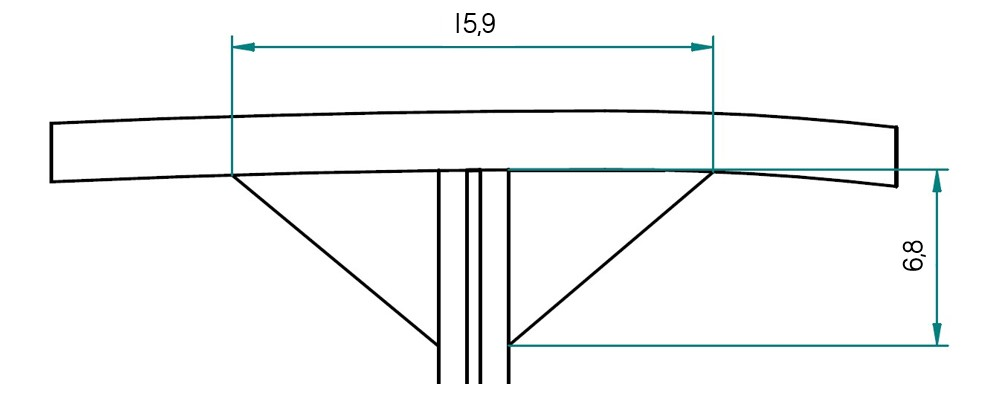
\includegraphics[width=0.75\textwidth]{Bilder/Mumpe.jpg}
	\centering
	\caption{Verklebung von Steg und Gurt}
	\label{fig: Mumpe}
\end{figure}

\noindent Abschließend wird die Gesamtmasse aus der Summe der einzelnen Massen berechnet. Sie ergibt sich zu:
\begin{equation}
\begin{array}{l}
	m_{ges}= m_{Gurt,o}+m_{Gurt,u}+m_{Steg,Verb}+m_{Steg,Schaum} \\ +m_{Haut,Schaum}+m_{Haut,innen}+m_{Haut,aussen} \\ +2\cdot m_{Rippe}+2\cdot m_{Klotz} \\
	+2\cdot m_{Haupthuelse}+2\cdot m_{Querhuelse}+2\cdot m_{Endhuelse}\\
	+m_{frei,o}+m_{frei,u}+m_{Kleber}\\
	=0,366kg
\end{array}  
\end{equation}
Die Gewichtslimitierung von 0,75kg wird eingehalten.

